\documentclass[12pt]{article}
\usepackage{fontspec}
\usepackage{adjustbox}
\usepackage{fancyvrb}
\usepackage{fancyhdr}
\usepackage{verbatim}
\usepackage{parskip}
\usepackage{amsmath}
\usepackage{tikz}
\usepackage{mathpazo}
\usepackage{sectsty}
\usepackage[T1]{fontenc}
\usepackage[a4paper, margin=2.5cm, headheight=35pt]{geometry}

\newenvironment{tabularverbatim}
{\VerbatimEnvironment
\begin{BVerbatim}[baseline=t]}
{\vspace{0.75em}\end{BVerbatim}}

\setlength{\parindent}{0pt}
\setlength{\parskip}{1em}

\setmonofont{Cascadia Mono}
\setsansfont{Inter}

\pagestyle{fancy}
% Redefine the fancy page style
\rhead{}
\lhead{\includegraphics[width=\textwidth]{header}}

\title{\textbf{Let's play \textit{osu!mania}}}
\author{\texttt{sahuang}}
\date{}
    
\usetikzlibrary{positioning}

\pgfdeclarehorizontalshading{whiteBg}{4cm}{color(0cm)=(black!10); 
color(1.99cm)=(white); 
color(2cm)=(black!15);color(4cm)=(black!10)}

\pgfdeclarehorizontalshading{redBg}{4cm}{color(0cm)=(red!40!black); 
color(1.99cm)=(red!5!white);
color(2cm)=(red!25!white);color(4cm)=(red!40!black)}

\pgfdeclarehorizontalshading{redBar}{4cm}{color(0cm)=(red!40!black); 
color(2cm)=(red!25!white);color(4cm)=(red!40!black)}
    
\begin{document}
\allsectionsfont{\bfseries\sffamily}
\maketitle
\thispagestyle{fancy}

\section{Problem Statement}

\begin{figure}[h]
    \centering

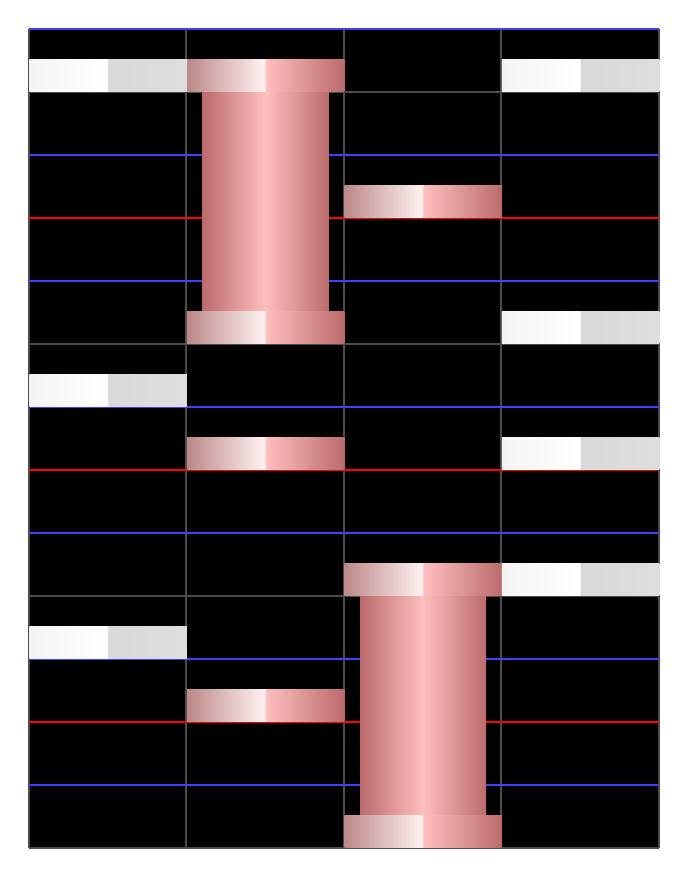
\begin{tikzpicture}[
	scale=2, yscale=0.4, 
	whiteNote/.style={rectangle,shading=whiteBg,minimum width=2cm,minimum height=0.4cm,anchor=south west},
	redNote/.style={rectangle,shading=redBg,minimum width=2cm,minimum height=0.4cm,anchor=south west},
	redHold/.style={rectangle,shading=redBar,minimum width=1.6cm,minimum height=0.4cm,anchor=south west},
]
	\fill[fill=black] (0,0) rectangle (4,13);
    \draw[thick,xstep=1cm,ystep=1cm,draw=white!30!black] (0,0) grid (4,13);
    \foreach \x in {1,3,...,13}{ \draw[thick,color=blue!75!white](0,\x) -- (4,\x); }
    \foreach \x in {2,6,...,10}{ \draw[thick,color=red](0,\x) -- (4,\x); }
	\node[redHold,minimum height=3.5cm] (n1) at (2.1,0) {};
	\node[redNote] (n1) at (2,0) {};
	\node[redNote] (n1) at (2,4) {};
	\node[redNote] (n1) at (1,2) {};
	\node[whiteNote] (n1) at (0,3) {};
	\node[whiteNote] (n1) at (3,4) {};
	\node[redNote] (n1) at (1,6) {};
	\node[whiteNote] (n1) at (3,6) {};
	\node[whiteNote] (n1) at (0,7) {};
	\node[whiteNote] (n1) at (3,8) {};
	\node[redHold,minimum height=3.5cm] (n1) at (1.1,8) {};
	\node[redNote] (n1) at (1,8) {};
	\node[redNote] (n1) at (1,12) {};
	\node[redNote] (n1) at (2,10) {};
	\node[whiteNote] (n1) at (0,12) {};
	\node[whiteNote] (n1) at (3,12) {};
\end{tikzpicture}

    \caption{\textit{osu!mania beatmap}}
    \label{fig:osumania}
\end{figure}

\textit{Miku} has been practising \textit{osu!mania 4K} for a while. It is a 4-key rhythm game where players will play a \textit{beatmap} by pressing the correct key for that specific note in time.

There are two types of objects in an \textit{osu!mania} beatmap:

\begin{enumerate}
    \item \textbf{Tap notes}: The falling notes must be tapped on the judgement line, with correct key corresponding to each of the note it falls to.

    \item \textbf{Hold notes}: When the hold note reaches the judgement line, tap the starting note in time with correct key, hold, and release it at the ending note of the hold note.
\end{enumerate}
Given a valid 4K beatmap, \textit{Miku} has asked you to calculate how many objects are there in this beatmap.

\section{Input}

The first line of input contains an integer $N$ ($10 \leq N \leq 10,000$), which corresponds to the length of the beatmap (i.e.~number of lines as shown in Figure \ref{fig:osumania}).

The next $N$ lines describe the beatmap. Each line is a string of length 6 where first and last character is guaranteed to be a vertical bar (``\texttt{|}''). The other 4 characters can be one of the following:

\begin{enumerate}
\item A single space (``\enskip'') meaning there is no note

\item A hyphen (``\texttt{-}'') meaning this is either a tap note or the beginning/ending of a hold note

\item A pound sign (``\texttt{\#}'') meaning it's the body of a hold note
\end{enumerate}
\textbf{It is guaranteed that the beatmap is valid}, i.e.~no overlapping notes or broken hold notes. Each hold note will have a beginning note ``\texttt{-}'', at least one body ``\texttt{\#}'' and an ending note ``\texttt{-}''.

\section{Output}

Output a single integer representing the total number of objects (tap notes + hold notes) in the beatmap.

\section{Sample}

\begin{center}
\def\arraystretch{1.8}%
\begin{tabular}{|p{0.47\textwidth}|p{0.47\textwidth}|}
\hline
Sample Input & Sample Output\\
\hline
\begin{tabularverbatim}
13
|-- -|
| #  |
| #- |
| #  |
| - -|
|-   |
| - -|
|    |
|  --|
|- # |
| -# |
|  # |
|  - |
\end{tabularverbatim}
&
\begin{tabularverbatim}
12
\end{tabularverbatim}
\\ \hline
\end{tabular}

\vspace{20pt}

\end{center}

\section{Explanation}

There is a total of 12 objects as shown in Figure \ref{fig:osumaniasol}.

\begin{figure}[h]
    \centering

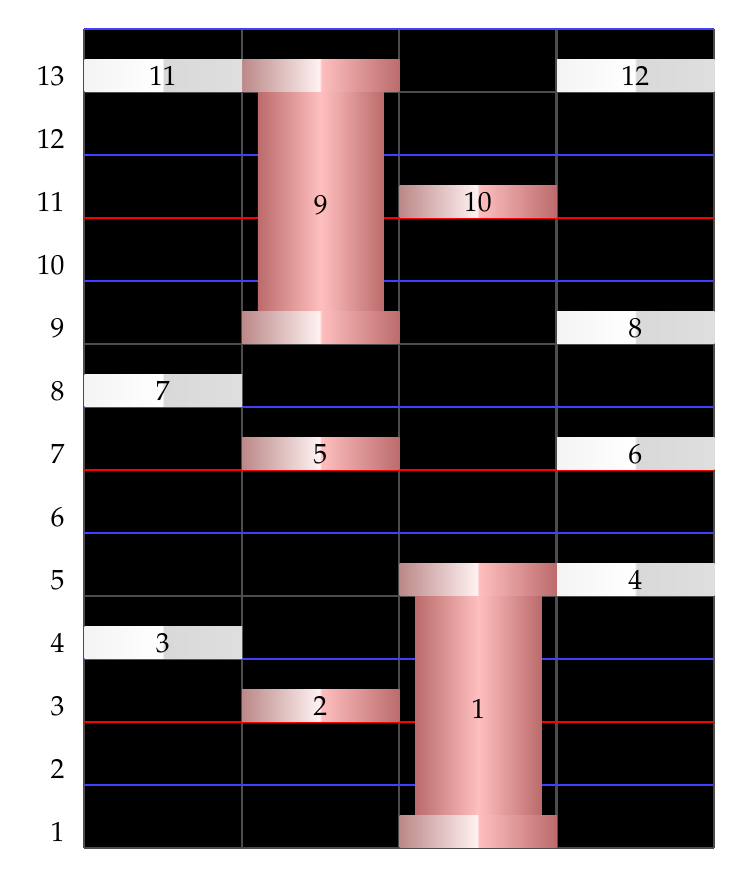
\begin{tikzpicture}[
	scale=2, yscale=0.4, 
	whiteNote/.style={rectangle,shading=whiteBg,minimum width=2cm,minimum height=0.4cm,anchor=south west,font=\tiny},
	redNote/.style={rectangle,shading=redBg,minimum width=2cm,minimum height=0.4cm,anchor=south west,font=\tiny},
	redHold/.style={rectangle,shading=redBar,minimum width=1.6cm,minimum height=0.4cm,anchor=south west},
]
	\fill[fill=black] (0,0) rectangle (4,13);
    \draw[thick,xstep=1cm,ystep=1cm,draw=white!30!black] (0,0) grid (4,13);
    \foreach \x in {1,3,...,13}{ \draw[thick,color=blue!75!white](0,\x) -- (4,\x); }
    \foreach \x in {2,6,...,10}{ \draw[thick,color=red](0,\x) -- (4,\x); }
	\node[redHold,minimum height=3.5cm] (note) at (2.1,0) {1};
	\node[redNote] (note) at (2,0) {};
	\node[redNote] (note) at (2,4) {};
	\node[redNote] (note2) at (1,2) {};
    \node[below left=-0.2 and -1 of note2,anchor=center] {2};
	\node[whiteNote] (note3) at (0,3) {};
    \node[below left=-0.2 and -1 of note3,anchor=center] {3};
	\node[whiteNote] (note4) at (3,4) {};
    \node[below left=-0.2 and -1 of note4,anchor=center] {4};
	\node[redNote] (note5) at (1,6) {};
    \node[below left=-0.2 and -1 of note5,anchor=center] {5};
	\node[whiteNote] (note6) at (3,6) {};
    \node[below left=-0.2 and -1 of note6,anchor=center] {6};
	\node[whiteNote] (note7) at (0,7) {};
    \node[below left=-0.2 and -1 of note7,anchor=center] {7};
	\node[whiteNote] (note8) at (3,8) {};
    \node[below left=-0.2 and -1 of note8,anchor=center] {8};
	\node[redHold,minimum height=3.5cm] (note) at (1.1,8) {9};
	\node[redNote] (note) at (1,8) {};
	\node[redNote] (note) at (1,12) {};
	\node[redNote] (note10) at (2,10) {};
    \node[below left=-0.2 and -1 of note10,anchor=center] {10};
	\node[whiteNote] (note11) at (0,12) {};
    \node[below left=-0.2 and -1 of note11,anchor=center] {11};
	\node[whiteNote] (note12) at (3,12) {};
    \node[below left=-0.2 and -1 of note12,anchor=center] {12};
	\foreach \x in {1,...,13}{\node[label=left:\x] at (0, \x-0.75) {};}
\end{tikzpicture}

    \caption{\textit{Beatmap} explained}
    \label{fig:osumaniasol}
\end{figure}

\end{document}
